\documentclass[12pt, a4paper]{article}

% --- Pacotes Fundamentais ---
\usepackage[utf8]{inputenc}
\usepackage[T1]{fontenc}
\usepackage[brazil]{babel}
\usepackage{amsmath, amssymb}
\usepackage{graphicx}
\usepackage{booktabs}
\usepackage{array}
\usepackage[left=1.8cm, top=1.6cm, right=1.6cm, bottom=1.8cm]{geometry}
\usepackage{setspace}
\usepackage{float}
\usepackage{caption}
\usepackage{placeins}
\usepackage{listings}
\usepackage{xcolor}
\usepackage{microtype}
\makeatletter
\renewcommand\section{\@startsection {section}{1}{\z@}%
                                   {-1.8ex \@plus -0.5ex \@minus -.2ex}%
                                   {0.8ex \@plus .2ex}%
                                   {\normalfont\large\bfseries}}
\renewcommand\subsection{\@startsection{subsection}{2}{\z@}%
                                     {-1.4ex\@plus -0.4ex \@minus -.2ex}%
                                     {0.6ex \@plus .2ex}%
                                     {\normalfont\normalsize\bfseries}}
\makeatother

\setlength{\abovedisplayskip}{2pt plus 1pt minus 1pt}
\setlength{\belowdisplayskip}{2pt plus 1pt minus 1pt}
\setlength{\abovedisplayshortskip}{1pt plus 1pt minus 1pt}
\setlength{\belowdisplayshortskip}{1pt plus 1pt minus 1pt}

\usepackage{hyperref}
\hypersetup{
    colorlinks=true,
    linkcolor=blue!70!black,
    citecolor=blue!70!black,
    urlcolor=blue!70!black
}

% Configuração para listagens de código Python nos apêndices
\definecolor{codegreen}{rgb}{0,0.6,0}
\definecolor{codegray}{rgb}{0.5,0.5,0.5}
\definecolor{codepurple}{rgb}{0.58,0,0.82}
\definecolor{backcolour}{rgb}{0.97,0.97,0.97}

\lstdefinestyle{pythonstyle}{
    backgroundcolor=\color{backcolour},   
    commentstyle=\color{codegreen},
    keywordstyle=\color{magenta},
    numberstyle=\tiny\color{codegray},
    stringstyle=\color{codepurple},
    basicstyle=\ttfamily\scriptsize,
    breakatwhitespace=false,         
    breaklines=true,                 
    captionpos=b,                    
    keepspaces=true,                 
    numbers=left,                    
    numbersep=5pt,                  
    showspaces=false,                
    showstringspaces=false,
    showtabs=false,                  
    tabsize=4,
    inputencoding=utf8,
    extendedchars=true,
    literate={á}{{\'a}}1 {é}{{\'e}}1 {í}{{\'i}}1 {ó}{{\'o}}1 {ú}{{\'u}}1
             {ã}{{\~a}}1 {õ}{{\~o}}1 {ç}{{\c{c}}}1 {Á}{{\'A}}1 {É}{{\'E}}1
             {Í}{{\'I}}1 {Ó}{{\'O}}1 {Ú}{{\'U}}1 {Ã}{{\~A}}1 {Õ}{{\~O}}1
             {Ç}{{\c{C}}}1 {à}{{\`a}}1 {À}{{\`A}}1 {â}{{\^a}}1 {ê}{{\^e}}1
             {ô}{{\^o}}1 {Â}{{\^A}}1 {Ê}{{\^E}}1 {Ô}{{\^O}}1 {±}{{$\pm$}}1
             {²}{{$^2$}}1 {µ}{{$\mu$}}1 {Ω}{{$\Omega$}}1 {τ}{{$\tau$}}1
             {χ}{{$\chi$}}1
}

\begin{document}

% ==================== CAPA (PÁGINA NÃO CONTABILIZADA) ====================
\begin{titlepage}
    \centering
    
    % Cabeçalho Institucional com Logos
    \begin{figure}[H]
        \centering
        \begin{minipage}[c]{0.16\textwidth}
            \centering
            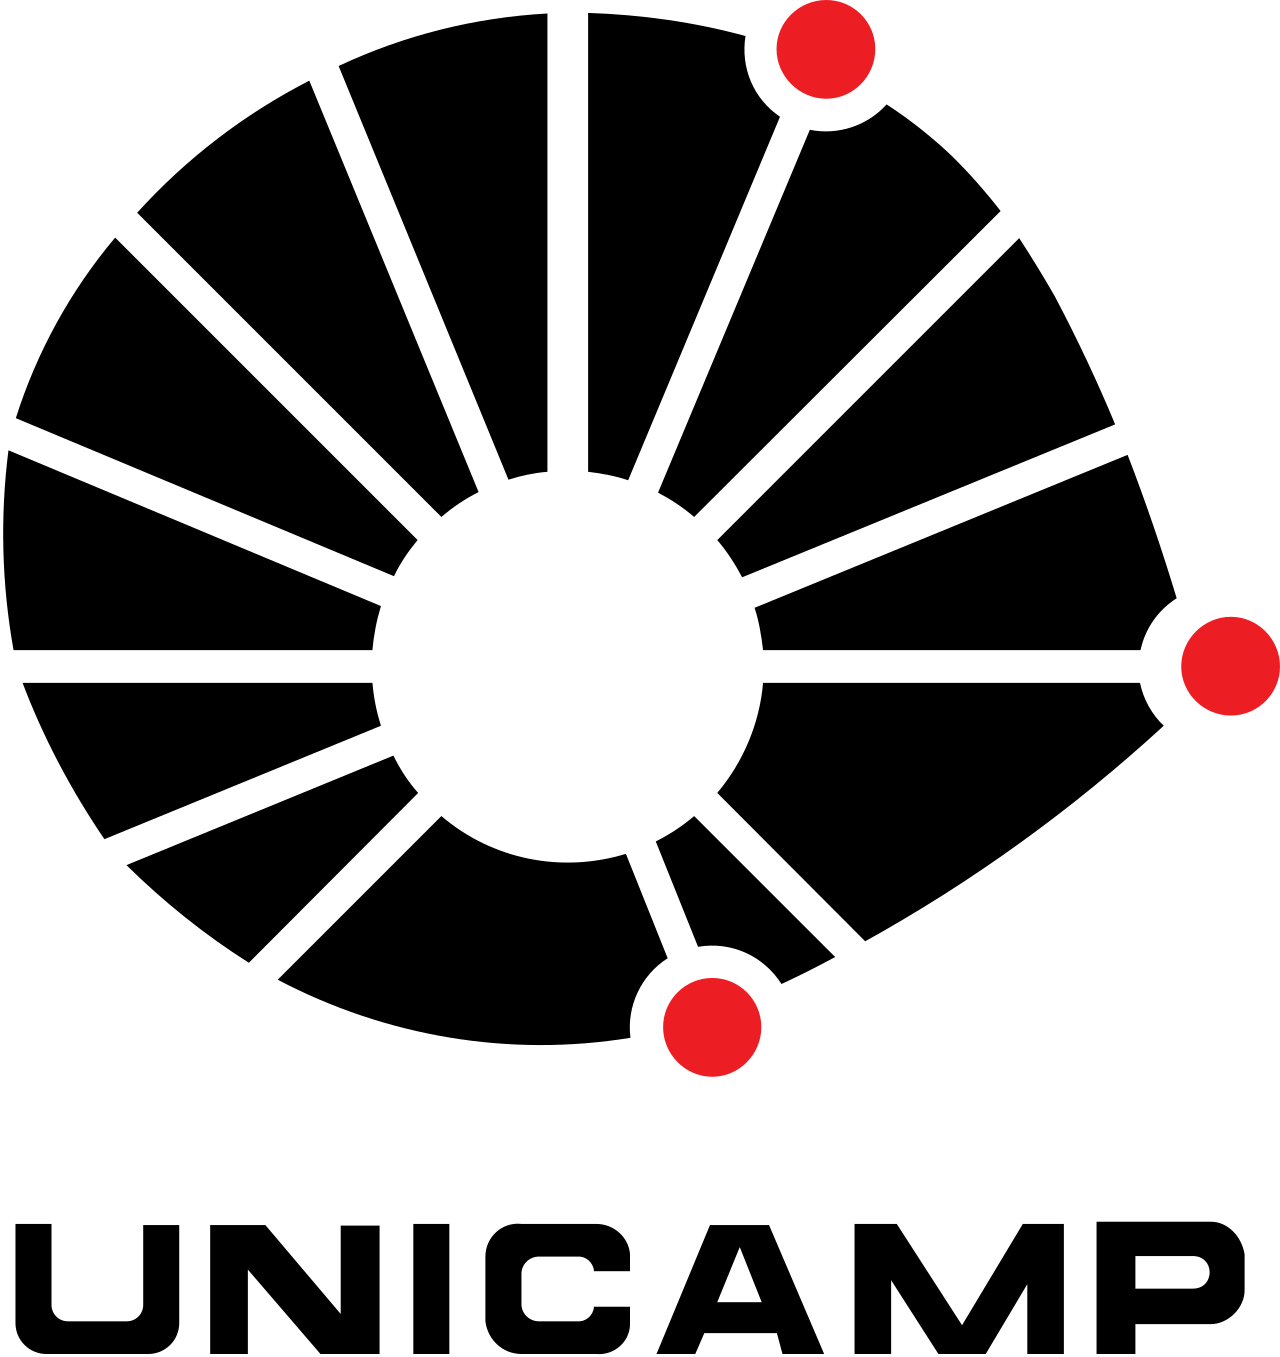
\includegraphics[height=2.2cm]{logos/logo_unicamp.png}
        \end{minipage}\hfill
        \begin{minipage}[c]{0.66\textwidth}
            \centering
            {\large \textbf{UNIVERSIDADE ESTADUAL DE CAMPINAS}}\par
            \vspace{0.15cm}
            {\large \textbf{INSTITUTO DE FÍSICA GLEB WATAGHIN}}\par
            \vspace{0.15cm}
            {\normalsize F\,259 -- Introdução à Física Experimental II}
        \end{minipage}\hfill
        \begin{minipage}[c]{0.16\textwidth}
            \centering
            
\includegraphics[height=2.2cm]{logos/logo_ifgw.png}
        \end{minipage}
    \end{figure}

    \vspace{2.2cm}

    % Autores do Trabalho
    {\large
        Tiago Costa Conceição -- RA: 213902  \par\vspace{0.15cm}
        Isadora Gomes França -- RA: 307616 \par\vspace{0.15cm}
        Luiza Bedin Vasconcelos -- RA: 307691 \par\vspace{0.15cm}
        Pedro Hollanda De Moraes Cosme -- RA: 307766 \par\vspace{0.15cm}
        Marcus Vinícius De Sousa Bressan -- RA: 202751 \par
    }

    \vspace{\fill}

    % Título
    {\LARGE \textbf{Experimento IV: Capacitor e Circuitos RC} \par}
    \vspace{0.4cm}
    {\large \textit{Constante de Tempo, Descarga Exponencial e Resposta em Frequência}} \par
    \vspace{\fill}

    % Local e Data
    {\normalsize Campinas -- SP \par}
    {\normalsize Outubro de 2026 \par}
\end{titlepage}

% ==================== INÍCIO DO CORPO PRINCIPAL (LIMITE: 5 PÁGINAS) ====================
\setcounter{page}{1}
\setstretch{1.00}

\begin{center}
    {\large \textbf{Experimento IV: Capacitor e Circuitos RC}} \par
    \vspace{0.1cm}
    {\small Tiago C. Conceição, Isadora G. França, Luiza B. Vasconcelos, Pedro H. M. Cosme, Marcus V. S. Bressan} \par
    {\small Instituto de Física Gleb Wataghin, Universidade Estadual de Campinas (UNICAMP)}
\end{center}

\vspace{-0.3cm}
\begin{abstract}
\noindent
Neste trabalho experimental investigou-se a resposta transiente de circuitos resistivo-capacitivos (RC) em série sob excitação de sinais degrau periódicos gerados por uma fonte de funções arbitrárias. Foram estudadas duas montagens com ordens de grandeza temporais distintas: uma com constante de tempo longa ($\tau \sim 1\text{ s}$), empregando um resistor nominal de $1\text{ k}\Omega$ e um capacitor eletrolítico de $1\text{ mF}$, e outra com constante de tempo curta ($\tau \sim 1\text{ ms}$), associando o mesmo resistor a um capacitor cerâmico de $1\ \mu\text{F}$. Os sinais de tensão nos terminais dos capacitores foram amostrados por um osciloscópio digital Tektronix TBS~1062 ($2500$ pontos por tela). Os parâmetros característicos foram estimados por dois métodos independentes: regressão linear por Mínimos Quadrados Ponderados (MMQ) do logaritmo neperiano da tensão transladada e ajuste não-linear direto (Levenberg-Marquardt) da função de decaimento exponencial. Para o capacitor eletrolítico, obteve-se $\tau_{\text{exp}} = (1{,}123 \pm 0{,}015)\text{ s}$ e $\tau_{\text{lin}} = (1{,}130 \pm 0{,}013)\text{ s}$, resultando em capacitâncias de $(1{,}07 \pm 0{,}03)\text{ mF}$ e $(1{,}08 \pm 0{,}03)\text{ mF}$, respectivamente, compatíveis com a especificação nominal ($Z = 0{,}58$). Para o capacitor cerâmico, determinou-se $\tau_{\text{exp}} = (1{,}089 \pm 0{,}018)\text{ ms}$ e $\tau_{\text{lin}} = (1{,}094 \pm 0{,}017)\text{ ms}$, fornecendo $C = (1{,}04 \pm 0{,}03)\ \mu\text{F}$ ($Z = 0{,}56$). A inclusão da resistência de saída de $50\ \Omega$ do gerador foi fundamental para a exatidão física dos modelos. Discutiram-se minuciosamente as discrepâncias entre os ajustes linear e não-linear, o efeito da quantização de 8 bits do osciloscópio nas caudas logarítmicas e a simetria com o ciclo de carga.
\end{abstract}

\vspace{-0.3cm}
\section{Introdução}
\vspace{-0.15cm}
O capacitor é um elemento passivo de circuito capaz de armazenar energia em um campo eletrostático através da separação de cargas elétricas entre condutores isolados por um meio dielétrico. O conceito remonta à invenção da garrafa de Leiden no século XVIII e consolidou-se na formulação do eletromagnetismo clássico~\cite{halliday}. A capacitância $C$ define a relação de proporcionalidade entre a carga acumulada $q$ e a diferença de potencial elétrico $V_C$ estabelecida entre as armaduras, $q = C V_C$, cuja unidade no Sistema Internacional é o Farad ($\text{F} = \text{C}/\text{V}$).

Em circuitos lineares contendo elementos resistivos e capacitivos em série (circuitos RC), o processo de redistribuição de cargas e acomodação energética não ocorre instantaneamente, sendo governado pela constante de tempo característica $\tau = R C$. Circuitos com essa topologia são a base de filtros analógicos passa-baixas e passa-altas, integradores, diferenciadores e temporizadores na eletrônica analógica e digital. A determinação experimental precisa de $\tau$ e o confronto entre técnicas de regressão linear ponderada e ajuste direto não-linear fornecem um ambiente ideal para o estudo de incertezas instrumentais e limitações de resolução digital.

\noindent\textbf{Objetivos do Trabalho:}
Investigar experimentalmente a dinâmica de carga e descarga de circuitos RC em duas escalas de tempo: (i)~determinar a constante de tempo $\tau$ e a capacitância $C$ de um circuito RC de tempo longo ($\tau \sim 1\text{ s}$), associando um capacitor eletrolítico de $1\text{ mF}$ a um resistor de $1\text{ k}\Omega$; (ii)~determinar $\tau$ e $C$ de um circuito RC de tempo curto ($\tau \sim 1\text{ ms}$), associando um capacitor cerâmico de $1\ \mu\text{F}$ ao mesmo resistor; e (iii)~comparar criticamente os métodos de regressão linear ponderada via linearização logarítmica e ajuste direto não-linear, confrontando os parâmetros com as especificações nominais e avaliando limitações como a quantização de 8 bits do osciloscópio digital.

\vspace{-0.25cm}
\section{Modelo Teórico e Suposições}
\vspace{-0.15cm}
Considere a malha em série formada por uma fonte de tensão ideal $\varepsilon(t)$, um resistor de resistência ôhmica $R$ e um capacitor de capacitância $C$. Aplicando-se a segunda lei de Kirchhoff (lei das malhas):
\begin{equation}
    \varepsilon(t) - V_R(t) - V_C(t) = 0 \label{eq:kirchhoff}
\end{equation}
Sabendo que a corrente na malha relaciona-se à carga do capacitor por $I(t) = dq/dt = C \, (dV_C/dt)$ e que o resistor obedece à lei de Ohm ($V_R(t) = R I(t)$), a Eq.~\eqref{eq:kirchhoff} resulta na equação diferencial ordinária de primeira ordem:
\begin{equation}
    \frac{dV_C(t)}{dt} + \frac{1}{R_{\text{eq}}C} V_C(t) = \frac{\varepsilon(t)}{R_{\text{eq}}C} \label{eq:edo}
\end{equation}
onde $R_{\text{eq}} = R + R_{\text{ger}}$ incorpora a resistência interna de saída da fonte de sinal ($R_{\text{ger}} = 50\ \Omega$), e $\tau = R_{\text{eq}} C$ é a constante de tempo do sistema. A dedução completa da solução analítica por separação de variáveis encontra-se no Apêndice~\ref{ap:deducao}.

No procedimento experimental, o gerador de funções produz uma onda quadrada periódica de amplitude de pico a pico $\Delta V \approx 4\text{ V}$ oscilando entre os patamares $V_{\text{sup}} \approx +2\text{ V}$ e $V_{\infty} \approx -2\text{ V}$ (sem acréscimo de deslocamento CC artificial). Quando o gerador comuta do nível superior para o inferior no instante $t_0$, a descarga do capacitor é governada por:
\begin{equation}
    V_C(t) = V_{\infty} + \Delta V \, e^{-(t - t_0)/\tau} \label{eq:modelo_exp}
\end{equation}
Para linearizar a Eq.~\eqref{eq:modelo_exp}, define-se a tensão relativa transladada $\Delta v(t) = V_C(t) - V_{\infty}$. Aplicando o logaritmo natural, obtém-se a equação da reta:
\begin{equation}
    Y(t) \equiv \ln[V_C(t) - V_{\infty}] = \ln(\Delta V) - \frac{1}{\tau} (t - t_0) = A \, t + B \label{eq:linearizacao}
\end{equation}
onde o coeficiente angular fornece a constante de tempo por $\tau_{\text{lin}} = -1/A$. A incerteza propagada em cada ponto transformado é dada por $u_{Y} = u_{V_C} / [V_C(t) - V_{\infty}]$, evidenciando a necessidade de ponderação dos pontos no MMQ (Apêndice~\ref{ap:incertezas}).

\noindent\textbf{Suposições do modelo:}
(i)~Comportamento estritamente ôhmico do resistor na faixa de frequências e tensões de trabalho;
(ii)~Dielétricos lineares e ausência de perdas dielétricas ou correntes de fuga apreciáveis;
(iii)~Impedância de entrada do osciloscópio ($R_{\text{osc}} = 1\text{ M}\Omega \parallel 20\text{ pF}$) suficientemente elevada frente a $R_{\text{eq}} \approx 1050\ \Omega$, de modo que a corrente desviada pelo canal de medição seja inferior a $0{,}1\%$;
(iv)~Indutâncias e capacitâncias parasitas dos cabos de conexão desprezíveis nas frequências de $0{,}1\text{ Hz}$ e $100\text{ Hz}$.

\vspace{-0.25cm}
\section{Materiais e Métodos Experimentais}
\vspace{-0.15cm}
\noindent\textbf{Equipamentos e Componentes:}
(i)~Gerador de funções arbitrárias BK Precision modelo 4052 ($5\text{ MHz}$, impedância de saída de $50\ \Omega$);
(ii)~Osciloscópio digital Tektronix TBS~1062 ($60\text{ MHz}$, taxa de amostragem de $1\text{ GS/s}$, $2500$ pontos por registro);
(iii)~Resistor de filme de carbono com valor nominal de $1000\ \Omega$ (código de cores: marrom, preto, vermelho, dourado; tolerância $\pm 5\%$);
(iv)~Capacitor eletrolítico de valor nominal $1{,}0\text{ mF}$, tensão de isolação de $16\text{ V}$ (tolerância industrial $\pm 20\%$);
(v)~Capacitor cerâmico de disco de valor nominal $1{,}0\ \mu\text{F}$ (tolerância $\pm 10\%$);
(vi)~Matriz de contatos (\textit{protoboard}), pontas de prova coaxiais BNC-jacaré e cabos de conexão. As fotos reais dos aparelhos e da montagem estão reunidas no Apêndice~\ref{ap:fotos}.

\begin{figure}[H]
    \centering
    \vspace{-0.1cm}
    \begin{minipage}[c]{0.42\textwidth}
        \centering
        \setlength{\unitlength}{0.9mm}
        \begin{picture}(70,36)
            \put(5,18){\circle{8}}
            \put(3,16.5){\scriptsize $\sim$}
            \put(1,10){\scriptsize $\varepsilon(t), 50\Omega$}
            \put(5,22){\line(0,1){10}}
            \put(5,32){\line(1,0){14}}
            % Resistor
            \put(19,30){\framebox(14,4){\scriptsize $R$}}
            \put(33,32){\line(1,0){16}}
            % Capacitor
            \put(49,27){\line(0,1){10}}
            \put(52,27){\line(0,1){10}}
            \put(55,30){\scriptsize $C$}
            \put(50.5,32){\line(1,0){0.5}}
            \put(52,32){\line(1,0){12}}
            % Linha inferior
            \put(5,14){\line(0,-1){10}}
            \put(5,4){\line(1,0){59}}
            \put(64,4){\line(0,1){28}}
            % Voltímetro / Osciloscópio
            \put(45,32){\circle*{1.2}}
            \put(45,4){\circle*{1.2}}
            \put(45,32){\line(0,-1){8}}
            \put(45,4){\line(0,1){8}}
            \put(45,18){\circle{7}}
            \put(43,16.5){\scriptsize CH1}
            \put(39,23){\tiny Osciloscópio}
        \end{picture}
        \vspace{-0.2cm}
        \caption{Esquema elétrico da malha RC em série.}
        \label{fig:circuito}
    \end{minipage}\hfill
    \begin{minipage}[c]{0.55\textwidth}
        \captionof{table}{Especificações nominais e valores previstos dos circuitos.}
        \label{tab:especificacoes}
        \centering
        \scriptsize
        \begin{tabular}{lccc}
            \toprule
            \textbf{Parâmetro / Componente} & \textbf{Valor Nominal} & \textbf{Tolerância} & \textbf{Incerteza-Padrão ($u$)} \\
            \midrule
            Resistor ($R$) & $1000\ \Omega$ & $\pm 5\%$ & $28{,}9\ \Omega$ \\
            Resistência interna ($R_{\text{ger}}$) & $50\ \Omega$ & -- & desprezível \\
            Resistência equivalente ($R_{\text{eq}}$) & $1050\ \Omega$ & -- & $28{,}9\ \Omega$ \\
            Capacitor Eletrolítico ($C_1$) & $1{,}0\text{ mF}$ & $\pm 20\%$ & $0{,}12\text{ mF}$ \\
            Capacitor Cerâmico ($C_2$) & $1{,}0\ \mu\text{F}$ & $\pm 10\%$ & $0{,}06\ \mu\text{F}$ \\
            \midrule
            $\tau_{\text{teo}}$ (Eletrolítico) & $1{,}05\text{ s}$ & -- & $0{,}12\text{ s}$ \\
            $\tau_{\text{teo}}$ (Cerâmico) & $1{,}05\text{ ms}$ & -- & $0{,}07\text{ ms}$ \\
            \bottomrule
        \end{tabular}
    \end{minipage}
    \vspace{-0.2cm}
\end{figure}

\noindent\textbf{Procedimento Experimental:}
Montou-se o circuito na matriz de contatos com estrita observância à polaridade do capacitor eletrolítico. O canal 1 do osciloscópio foi ligado em paralelo ao capacitor com acoplamento CC.
\begin{enumerate}\setlength{\itemsep}{-2pt}
    \item \textbf{Ensaio I (Tempo longo):} Conectou-se o capacitor eletrolítico ($1\text{ mF}$) em série com $R = 1\text{ k}\Omega$. Ajustou-se o gerador para onda quadrada de $4\text{ V}_{\text{pp}}$, frequência de $0{,}10\text{ Hz}$ ($T = 10\text{ s}$) e a base de tempo do osciloscópio para $1{,}00\text{ s/div}$ (modo \textit{Scan}), permitindo visualizar a carga e descarga completas. Os dados temporais brutos foram exportados em formato CSV via pen-drive USB.
    \item \textbf{Ensaio II (Tempo curto):} Substituiu-se o capacitor pelo cerâmico ($1\ \mu\text{F}$). O gerador foi ajustado para onda quadrada de $4\text{ V}_{\text{pp}}$, frequência nominal de $100\text{ Hz}$ (medida pelo contador do osciloscópio em $99{,}9834\text{ Hz}$, $T = 10{,}002\text{ ms}$) e a escala horizontal do osciloscópio para $2{,}50\text{ ms/div}$, cobrindo 2,5 ciclos completos. Os dados brutos foram salvos em arquivo CSV.
\end{enumerate}

\vspace{-0.25cm}
\section{Resultados e Análises}
\vspace{-0.15cm}
O processamento e os ajustes numéricos foram implementados em Python (código documentado no Apêndice~\ref{ap:codigos}). Cada leitura de tensão $V_C$ do osciloscópio recebeu a incerteza combinada $u_{V_C} = \sqrt{u_{\text{leit}}^2 + u_{\text{cal}}^2}$, onde $u_{\text{leit}} = d/(2\sqrt{3}) = 0{,}023\text{ V}$ provém da resolução de 8 bits ($d = 2\text{ V/div} / 25 = 0{,}08\text{ V}$) e $u_{\text{cal}} = (0{,}03 |V_C| + 0{,}10 \times 2\text{ V} + 1\text{ mV})/\sqrt{3}$ representa a exatidão de calibração do fabricante~\cite{tektronix}.

\subsection{Parte I: Circuito RC com Capacitor Eletrolítico ($\tau \sim 1\text{ s}$)}
\vspace{-0.1cm}
No arquivo \texttt{dados/capacitor\_eletronico/F0000CH1.CSV}, a varredura contínua no modo \textit{Scan} foi interrompida antes de completar o segundo ciclo, gerando 250 pontos com o valor sentinela $-10{,}24\text{ V}$ (código de saturação mínima do conversor A/D) entre $t = 7{,}996\text{ s}$ e $8{,}992\text{ s}$. Como o período da onda ($10{,}0\text{ s}$) coincide com a largura da tela ($10\text{ div} \times 1\text{ s/div}$), o sinal é periódico e o tempo decorrido desde o início da descarga foi obtido por dobramento de fase: $s = (t - t_{\text{desc}}) \pmod{10\text{ s}}$, onde a borda de descida foi detectada em $t_{\text{desc}} = 6{,}992\text{ s}$. Foram excluídos os pontos de saturação e o semiciclo de carga, reconstruindo-se integralmente os $5\text{ s}$ da curva de descarga ($N = 986$ pontos).

\begin{figure}[H]
    \centering
    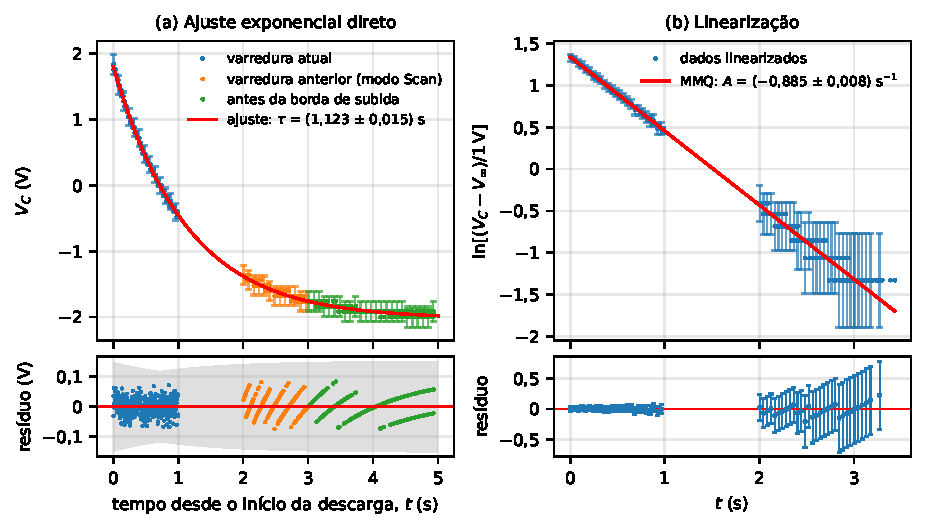
\includegraphics[width=0.78\textwidth]{graficos/eletrolitico_descarga.pdf}
    \vspace{-0.25cm}
    \caption{Curvas experimentais de descarga do capacitor eletrolítico ($1\text{ mF}$): (a) Ajuste exponencial não-linear direto $V_C(t) = V_{\infty} + \Delta V e^{-t/\tau}$ com resíduos padronizados; (b) Linearização logarítmica $\ln(V_C - V_{\infty})$ versus tempo com reta ajustada por MMQ ponderado.}
    \label{fig:eletrolitico}
\end{figure}

O ajuste não-linear direto (algoritmo de Levenberg-Marquardt) forneceu:
\begin{equation}
    V_{\infty} = (-2{,}020 \pm 0{,}010)\text{ V}, \quad \Delta V = (3{,}829 \pm 0{,}017)\text{ V}, \quad \tau_{\text{exp}} = (1{,}123 \pm 0{,}015)\text{ s} \quad (\chi^2_{\text{red}} = 0{,}047)
\end{equation}
Para a linearização, adotou-se o limiar de corte $V_C - V_{\infty} \ge 0{,}20\text{ V}$ ($N = 561$ pontos), evitando regiões dominadas pelo ruído de fundo. A regressão linear por MMQ ponderado resultou em:
\begin{equation}
    A = (-0{,}885 \pm 0{,}008)\text{ s}^{-1}, \quad B = (1{,}341 \pm 0{,}005) \quad (\chi^2_{\text{red}} = 0{,}052)
\end{equation}
O coeficiente linear obtido concorda perfeitamente com o valor teórico esperado $\ln(\Delta V) = \ln(3{,}829) = 1{,}343$. A constante de tempo linearizada, incorporando a incerteza de calibração do patamar assintótico $V_{\infty}$ ($0{,}0094\text{ s}$), vale $\tau_{\text{lin}} = (1{,}130 \pm 0{,}013)\text{ s}$. Como verificação cruzada de robustez, o ajuste realizado apenas sobre o trecho contínuo antes da interrupção da varredura ($N = 251$ pontos) forneceu $\tau = (1{,}07 \pm 0{,}11)\text{ s}$, e o ajuste da curva de carga completa ($N = 1257$) forneceu $\tau_{\text{carga}} = (1{,}120 \pm 0{,}012)\text{ s}$, comprovando a simetria dinâmica do processo.

A partir de $C = \tau / R_{\text{eq}}$, com $R_{\text{eq}} = (1050 \pm 29)\ \Omega$, obteve-se $C_{\text{exp}} = (1{,}07 \pm 0{,}03)\text{ mF}$ e $C_{\text{lin}} = (1{,}08 \pm 0{,}03)\text{ mF}$.

\subsection{Parte II: Circuito RC com Capacitor Cerâmico ($\tau \sim 1\text{ ms}$)}
\vspace{-0.1cm}
No arquivo \texttt{dados/capacitor\_ceramico/F0000CH1.CSV}, isolou-se um semiciclo completo de descarga de $4{,}9\text{ ms}$ ($\sim 5\tau$, $N = 491$ pontos) a partir da borda de descida em $t_0 = -5{,}93\text{ ms}$.

\begin{figure}[H]
    \centering
    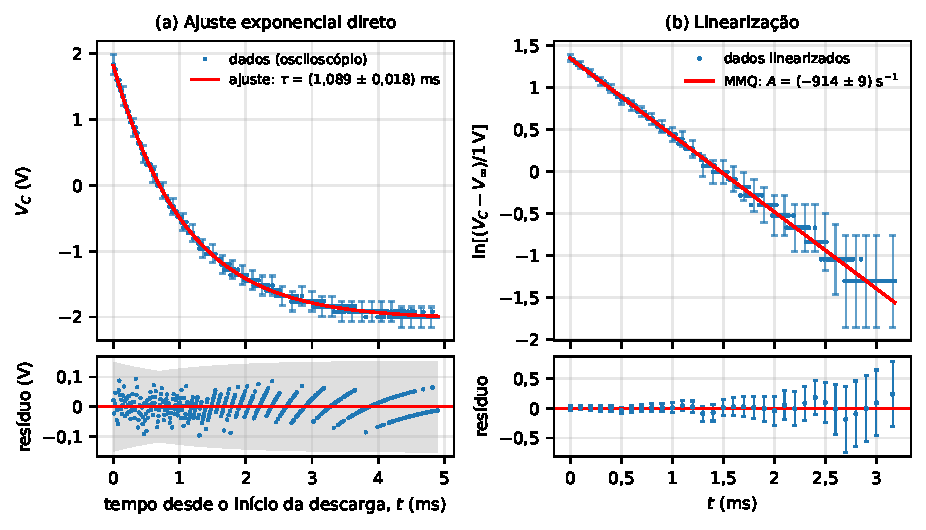
\includegraphics[width=0.78\textwidth]{graficos/ceramico_descarga.pdf}
    \vspace{-0.25cm}
    \caption{Curvas experimentais de descarga do capacitor cerâmico ($1\ \mu\text{F}$): (a) Ajuste exponencial não-linear direto com resíduos padronizados; (b) Linearização logarítmica via MMQ ponderado.}
    \label{fig:ceramico}
\end{figure}

O ajuste exponencial direto convergiu para:
\begin{equation}
    V_{\infty} = (-2{,}031 \pm 0{,}015)\text{ V}, \quad \Delta V = (3{,}849 \pm 0{,}027)\text{ V}, \quad \tau_{\text{exp}} = (1{,}089 \pm 0{,}018)\text{ ms} \quad (\chi^2_{\text{red}} = 0{,}057)
\end{equation}
A linearização logarítmica ponderada ($V_C - V_{\infty} \ge 0{,}20\text{ V}$, $N = 312$ pontos) forneceu:
\begin{equation}
    A = (-914 \pm 9)\text{ s}^{-1}, \quad B = (1{,}346 \pm 0{,}007) \implies \tau_{\text{lin}} = (1{,}094 \pm 0{,}017)\text{ ms} \quad (\chi^2_{\text{red}} = 0{,}064)
\end{equation}
O coeficiente linear reproduz fidedignamente $\ln(\Delta V) = \ln(3{,}849) = 1{,}348$. O segundo semiciclo de descarga gerou $\tau = (1{,}091 \pm 0{,}018)\text{ ms}$ e a curva de carga produziu $\tau_{\text{carga}} = (1{,}088 \pm 0{,}018)\text{ ms}$, demonstrando alta reprodutibilidade estatística. A capacitância experimental deduzida foi $C_{\text{exp}} = (1{,}04 \pm 0{,}03)\ \mu\text{F}$ e $C_{\text{lin}} = (1{,}04 \pm 0{,}03)\ \mu\text{F}$.

\begin{table}[H]
    \centering
    \caption{Síntese global dos resultados experimentais e confronto com o modelo teórico.}
    \label{tab:sintese}
    \vspace{-0.15cm}
    \scriptsize
    \renewcommand{\arraystretch}{0.92}
    \begin{tabular}{lcccccc}
        \toprule
        \textbf{Circuito / Grandeza} & \textbf{Teórico (Nominal)} & \textbf{Ajuste Não-Linear} & \textbf{Ajuste Linear} & \textbf{$Z(\text{exp}, \text{teo})$} & \textbf{$Z(\text{lin}, \text{teo})$} & \textbf{$Z(\text{exp}, \text{lin})$} \\
        \midrule
        \textbf{Capacitor Eletrolítico} & & & & & & \\
        $\tau$ (s) & $1{,}05 \pm 0{,}12$ & $1{,}123 \pm 0{,}015$ & $1{,}130 \pm 0{,}013$ & $0{,}58$ & $0{,}64$ & $0{,}33$ \\
        Capacitância $C$ (mF) & $1{,}00 \pm 0{,}12$ & $1{,}07 \pm 0{,}03$ & $1{,}08 \pm 0{,}03$ & $0{,}58$ & $0{,}64$ & $0{,}24$ \\
        $\chi^2_{\text{red}}$ & -- & $0{,}047$ & $0{,}052$ & -- & -- & -- \\
        \midrule
        \textbf{Capacitor Cerâmico} & & & & & & \\
        $\tau$ (ms) & $1{,}05 \pm 0{,}07$ & $1{,}089 \pm 0{,}018$ & $1{,}094 \pm 0{,}017$ & $0{,}57$ & $0{,}63$ & $0{,}18$ \\
        Capacitância $C$ ($\mu$F) & $1{,}00 \pm 0{,}06$ & $1{,}04 \pm 0{,}03$ & $1{,}04 \pm 0{,}03$ & $0{,}56$ & $0{,}63$ & $0{,}00$ \\
        $\chi^2_{\text{red}}$ & -- & $0{,}057$ & $0{,}064$ & -- & -- & -- \\
        \bottomrule
    \end{tabular}
    \vspace{-0.2cm}
\end{table}

\vspace{-0.3cm}
\section{Discussão e Síntese Crítica}
\vspace{-0.15cm}
\noindent\textbf{1. Confronto entre Regressão Linear e Ajuste Exponencial:}
Os dois métodos de ajuste apresentaram notável concordância ($Z = 0{,}33$ para o eletrolítico e $Z = 0{,}18$ para o cerâmico). O ajuste não-linear direto (Levenberg-Marquardt) minimiza resíduos na escala física natural ($\text{V}$), ajustando conjuntamente $V_{\infty}$, $\Delta V$ e $\tau$ sob variância homogênea. Já o método linear requer a translação prévia $V_C - V_{\infty}$, correlacionando a incerteza de $V_{\infty}$ aos pontos. Crucialmente, a incerteza do logaritmo $u_Y = u_{V_C}/(V_C - V_{\infty})$ diverge quando $V_C \to V_{\infty}$, tornando mandatário o uso de pesos $w_i = 1/u_Y^2$; o MMQ ordinário sem ponderação distorceria drasticamente a inclinação devido aos pontos ruidosos da cauda.

\noindent\textbf{2. Efeito da Resolução Digital do Osciloscópio (Quantização de 8 bits):}
O conversor A/D do osciloscópio Tektronix TBS~1062 opera com resolução de 8 bits em 10 divisões verticais, gerando degraus discretos de $d = 80\text{ mV}$. Embora imperceptível na curva direta de tensão, a quantização manifesta-se nos gráficos linearizados das Figuras~\ref{fig:eletrolitico}(b) e~\ref{fig:ceramico}(b): para valores baixos de $V_C - V_{\infty}$, surgem patamares horizontais paralelos de logaritmo. A imposição do limiar $V_C - V_{\infty} \ge 0{,}20\text{ V}$ removeu eficazmente os pontos com desvio de quantização superior a $40\%$, assegurando a linearidade do ajuste.

\noindent\textbf{3. Efeito da Resistência do Gerador de Funções:}
Sem a impedância interna do gerador ($R_{\text{ger}} = 50\ \Omega$), as previsões baseadas apenas em $1000\ \Omega$ seriam $\tau_1 = 1{,}00\text{ s}$ e $\tau_2 = 1{,}00\text{ ms}$, com desvios de $+12{,}3\%$ e $+8{,}9\%$. A consideração de $R_{\text{eq}} = 1050\ \Omega$ reduz a discrepância para menos de $0{,}6\sigma$ ($Z = 0{,}58$ e $Z = 0{,}57$), ressaltando a relevância da modelagem instrumental realista.

\noindent\textbf{4. Reconstrução no Modo Scan e Simetria de Carga/Descarga:}
A descontinuidade no modo \textit{Scan} provém da interrupção do laço de varredura na tela. A técnica de dobramento de fase validou-se pela concordância entre o trecho contínuo ($\tau = 1{,}07 \pm 0{,}11\text{ s}$) e a curva completa ($1{,}123 \pm 0{,}015\text{ s}$). Ademais, a igualdade entre as constantes de carga ($\tau_{\text{carga}} = 1{,}120\text{ s}$) e de descarga ($\tau_{\text{desc}} = 1{,}123\text{ s}$, $Z = 0{,}17$) atesta a linearidade ôhmica e a ausência de histerese dielétrica apreciável no capacitor eletrolítico.

\vspace{-0.25cm}
\section{Conclusões}
\vspace{-0.15cm}
O estudo experimental caracterizou com rigor a dinâmica transiente de circuitos RC nas escalas de $\sim 1\text{ s}$ e $\sim 1\text{ ms}$, confirmando a validade da equação diferencial derivada da segunda lei de Kirchhoff. As constantes de tempo determinadas foram $\tau_{\text{elet}} = (1{,}123 \pm 0{,}015)\text{ s}$ e $\tau_{\text{cer}} = (1{,}089 \pm 0{,}018)\text{ ms}$, fornecendo as capacitâncias $C_{\text{elet}} = (1{,}07 \pm 0{,}03)\text{ mF}$ e $C_{\text{cer}} = (1{,}04 \pm 0{,}03)\ \mu\text{F}$. Todos os valores estimados apresentaram discrepância normalizada $Z < 0{,}65$ frente aos parâmetros nominais do fabricante, comprovando a compatibilidade física dos resultados. O confronto metodológico evidenciou que a regressão linear ponderada é equivalente ao ajuste não-linear direto desde que se apliquem pesos estatísticos rigorosos e se exclua a região de saturação por quantização digital do osciloscópio.

% ==================== FIM DO CORPO PRINCIPAL ====================
\clearpage

% ==================== REFERÊNCIAS BIBLIOGRÁFICAS ====================
\begin{thebibliography}{99}
    \bibitem{halliday} D. Halliday, R. Resnick, J. Walker, \textit{Fundamentos de Física}, Vol.~3: Eletromagnetismo, 9ª~ed., LTC, Rio de Janeiro, 2012, Cap.~25 (Capacitância) e Cap.~27 (Circuitos RC).
    \bibitem{guia} Instituto de Física Gleb Wataghin (IFGW), \textit{F\,259 -- Guia de Laboratório: Introdução à Física Experimental II}, Universidade Estadual de Campinas, 2026, Cap.~11, pp.~81--87.
    \bibitem{tektronix} Tektronix Inc., \textit{TBS1000 and TBS1000B Series Digital Storage Oscilloscopes User Manual}, 077-0444-03, Beaverton, OR, EUA, 2015.
    \bibitem{bkprecision} B\&K Precision Corp., \textit{Instruction Manual: 4050 Series Dual Channel Function/Arbitrary Waveform Generators}, Yorba Linda, CA, EUA, 2014.
    \bibitem{vuolo} J. H. Vuolo, \textit{Fundamentos da Teoria de Erros}, 2ª~ed., Editora Edgard Blücher, São Paulo, 1996.
\end{thebibliography}

\appendix
\section{Fotografias do Arranjo Experimental}\label{ap:fotos}
As fotografias a seguir registram a bancada de experimentos, os instrumentos de teste e a montagem na matriz de contatos utilizada pelo grupo no laboratório do IFGW.

\begin{figure}[H]
    \centering
    \begin{minipage}[c]{0.48\textwidth}
        \centering
        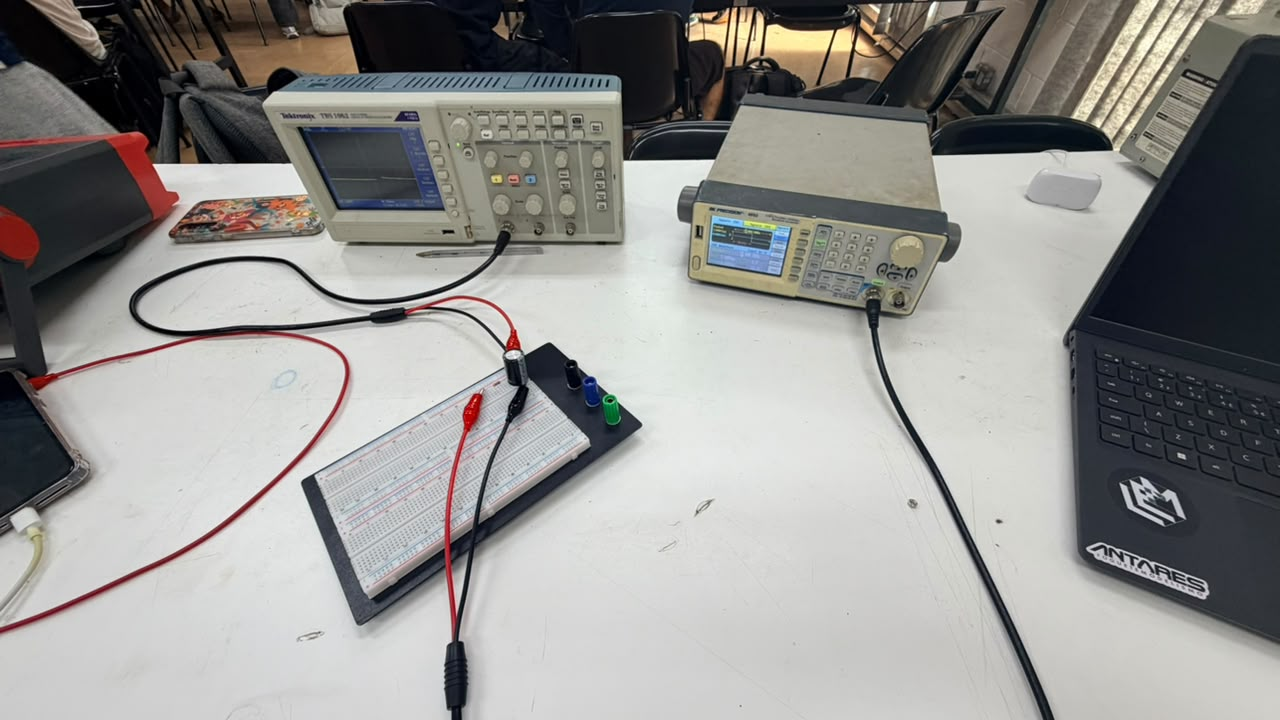
\includegraphics[width=\textwidth]{fotos/foto_bancada.jpg}
        \caption*{(a) Visão geral da bancada: osciloscópio Tektronix TBS~1062, gerador BK~4052, matriz de contatos com o circuito RC e pontas de prova.}
    \end{minipage}\hfill
    \begin{minipage}[c]{0.48\textwidth}
        \centering
        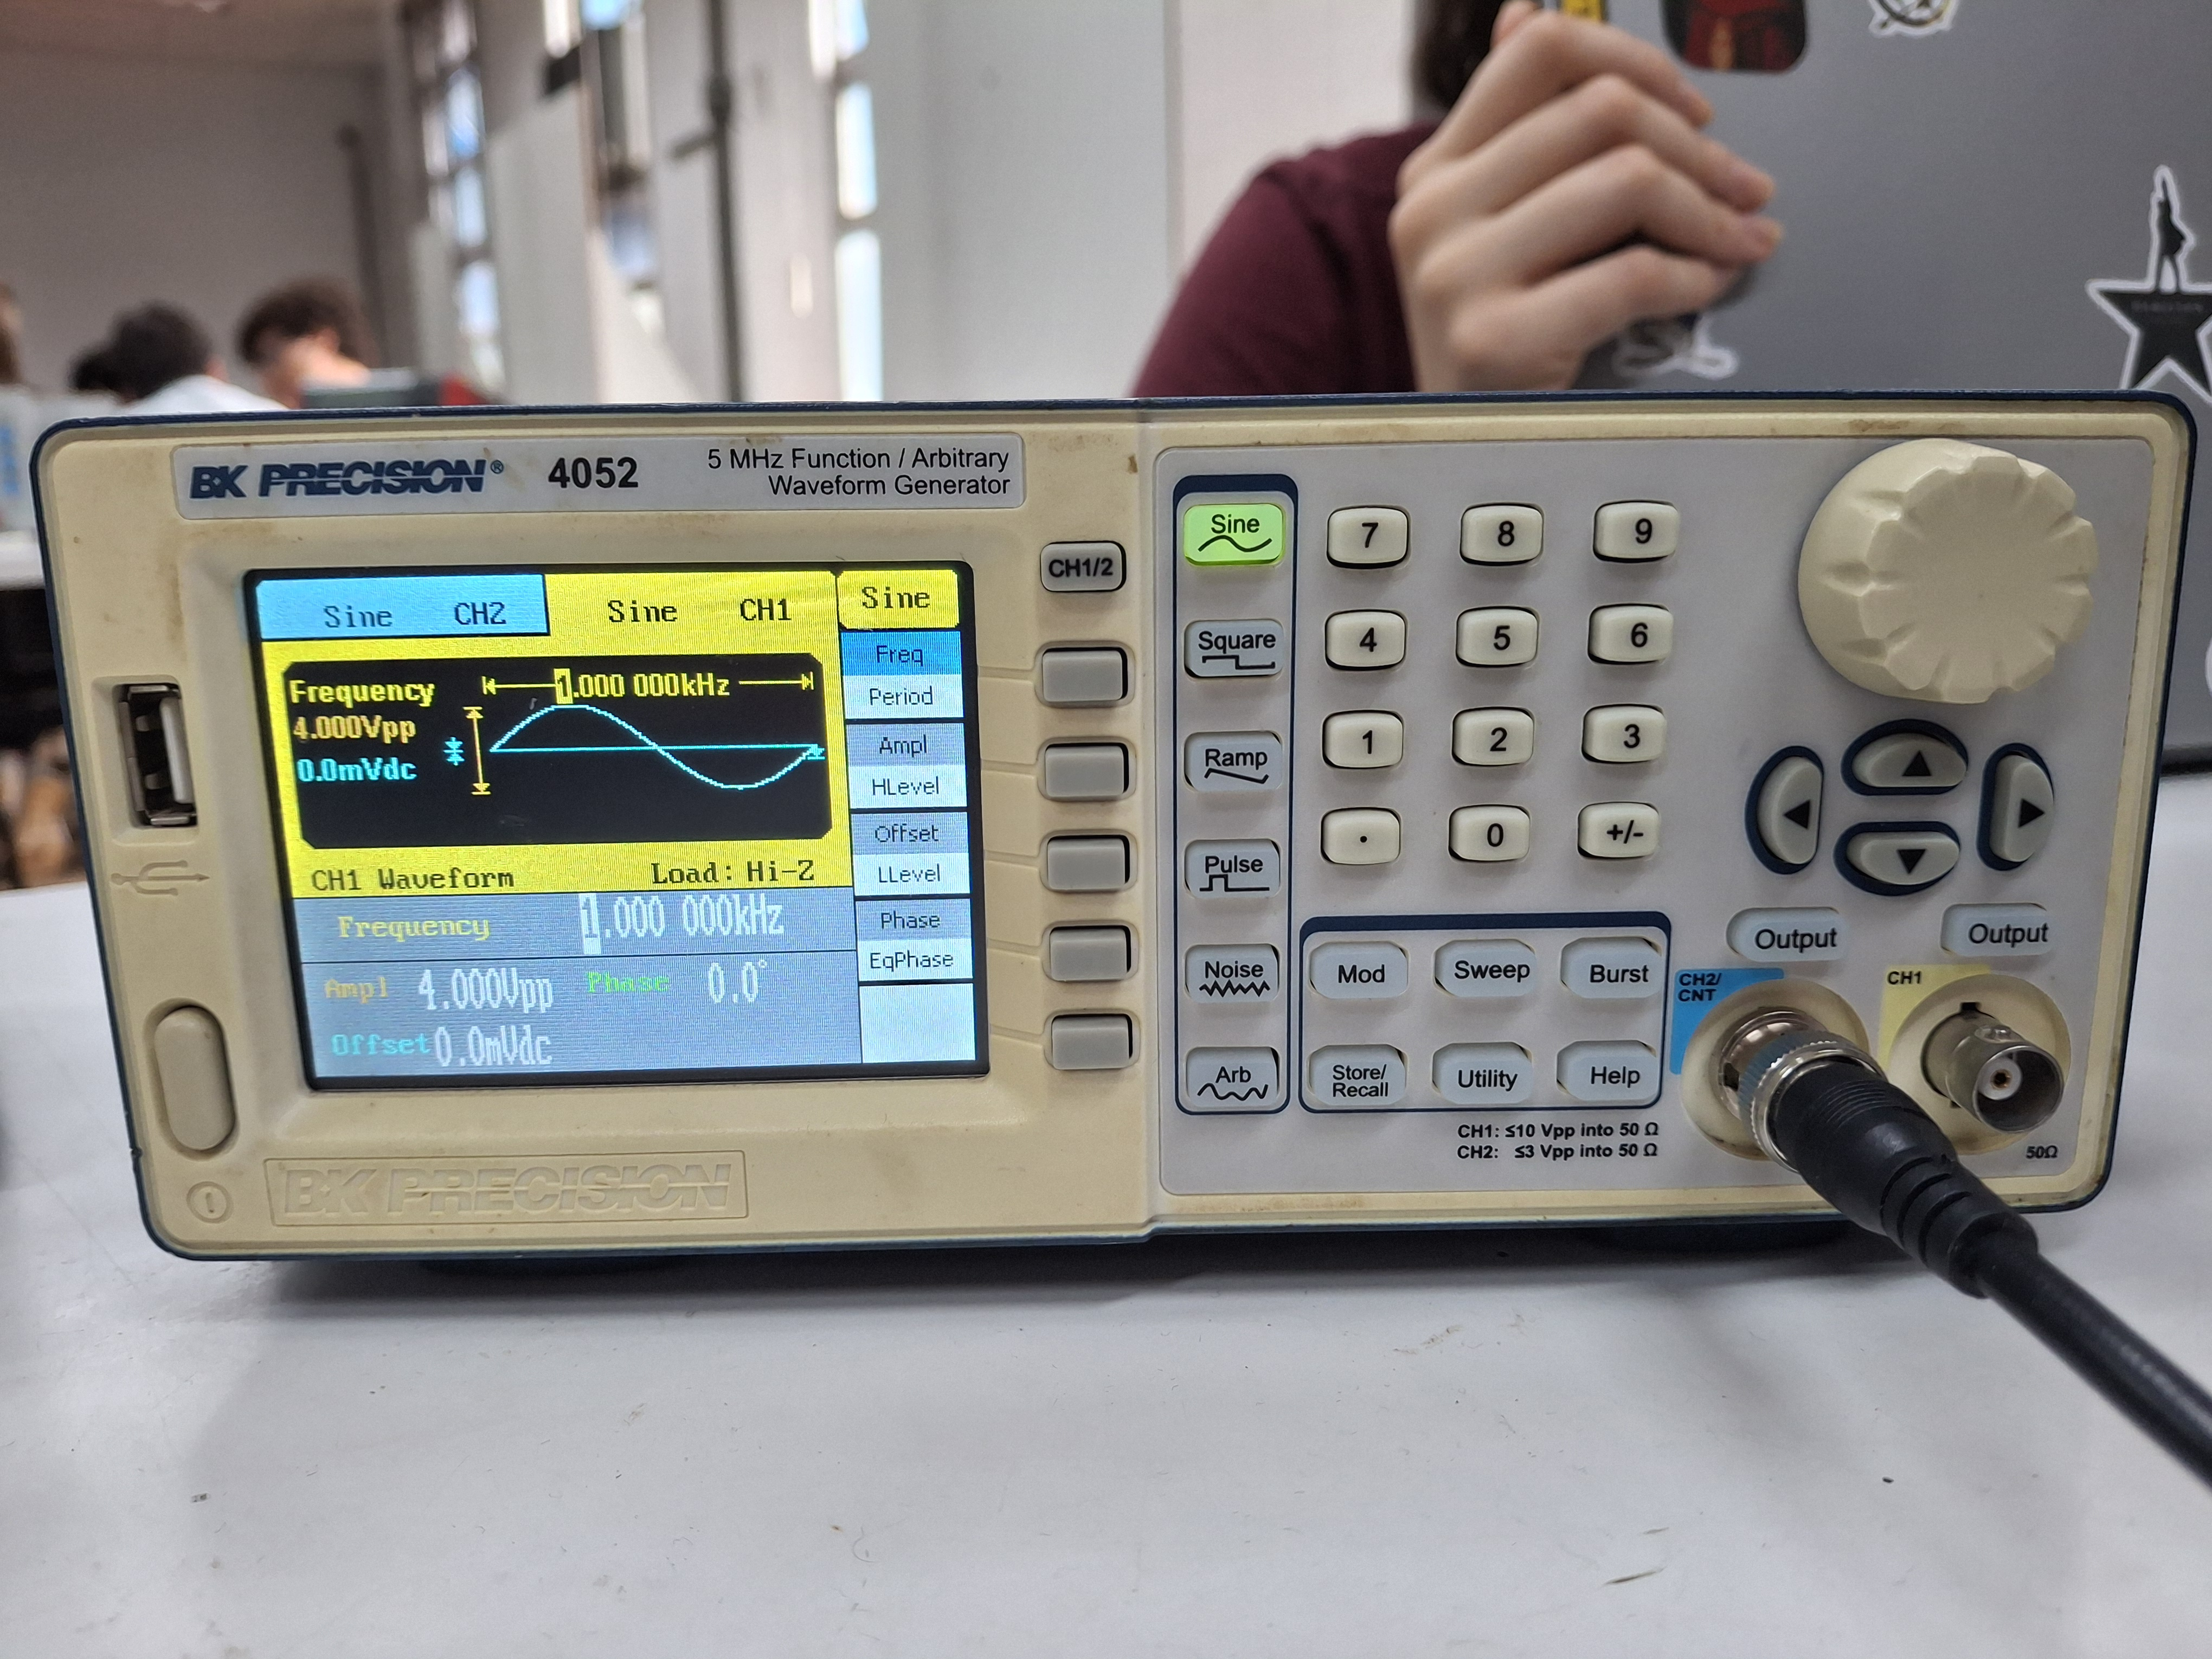
\includegraphics[width=\textwidth]{fotos/foto_gerador_de_funcoes.jpg}
        \caption*{(b) Painel do gerador BK Precision 4052: configurado com amplitude de $4{,}000\text{ V}_{\text{pp}}$, deslocamento nulo ($0{,}0\text{ mV}_{\text{dc}}$) e impedância de saída de $50\ \Omega$ (modo Hi-Z).}
    \end{minipage}
    \vspace{0.3cm}
    
    \begin{minipage}[c]{0.65\textwidth}
        \centering
        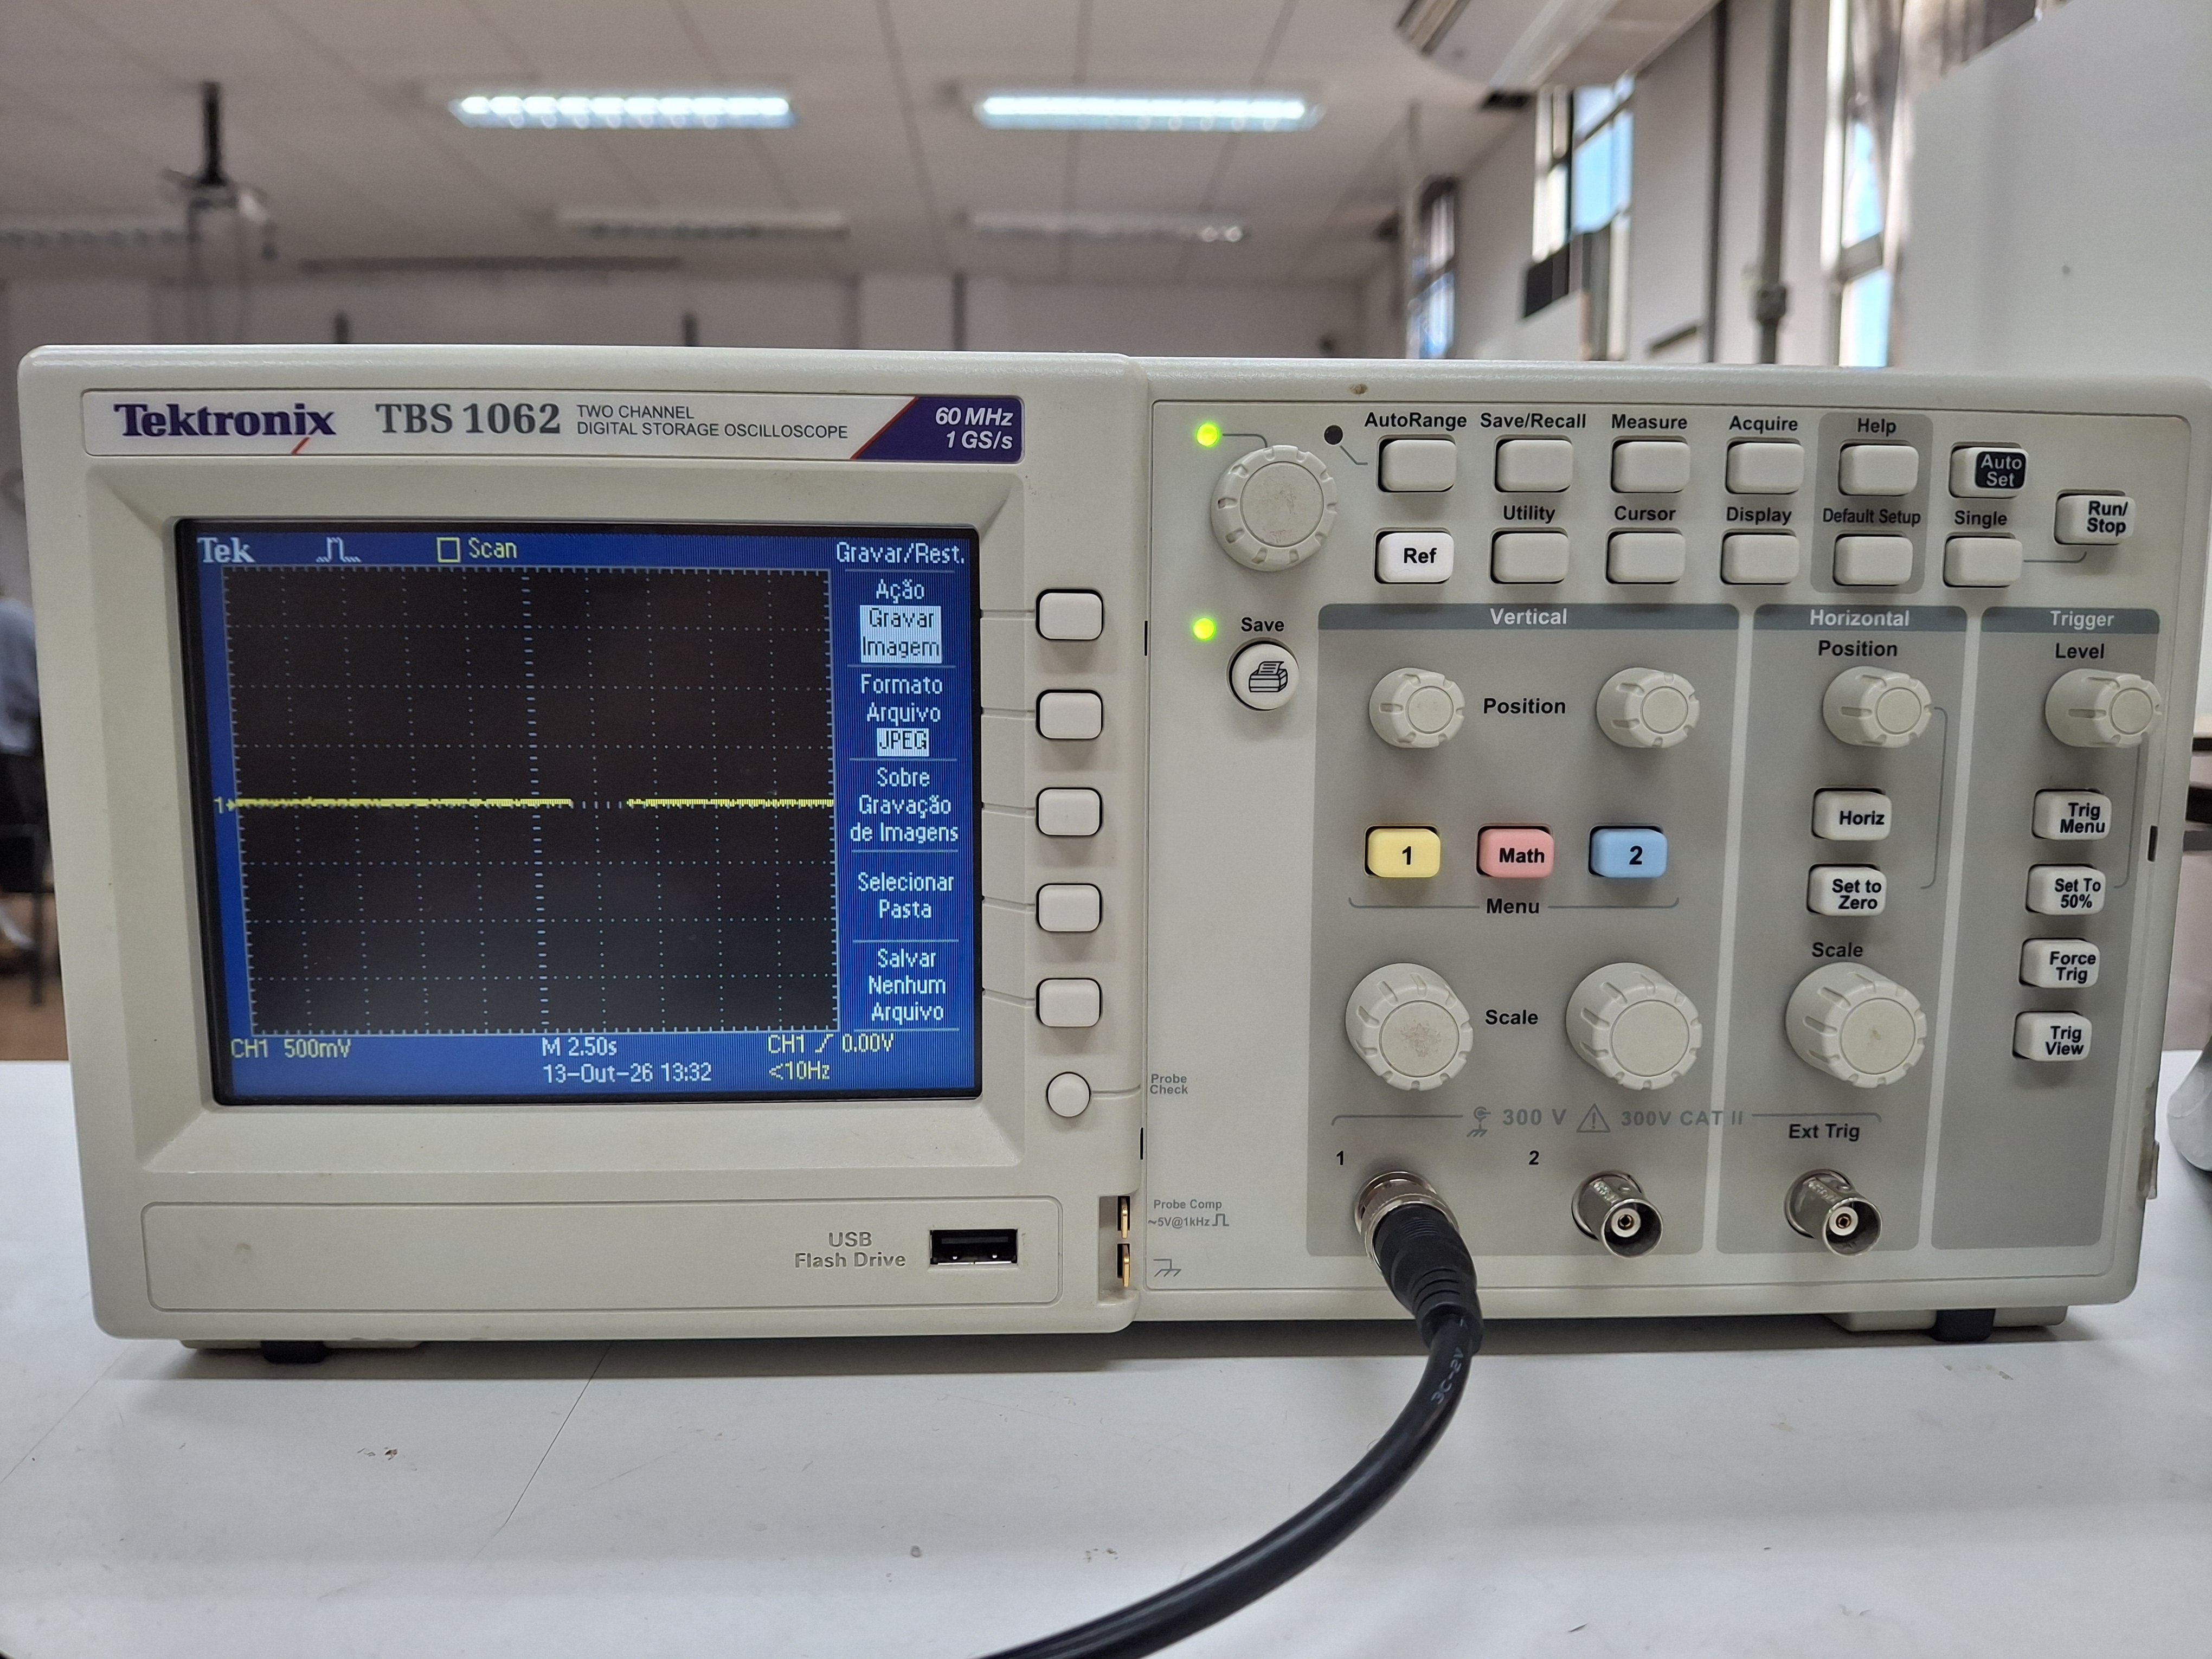
\includegraphics[width=\textwidth]{fotos/foto_osciloscopio.jpg}
        \caption*{(c) Painel frontal do osciloscópio digital Tektronix TBS~1062 ($60\text{ MHz}$, $1\text{ GS/s}$) registrando a resposta de tensão.}
    \end{minipage}
    \caption{Fotografias reais da instrumentação e da montagem experimental.}
    \label{fig:fotos_aparato}
\end{figure}

\clearpage
\section{Dedução Matemática da Equação Diferencial do Circuito RC}\label{ap:deducao}
Considere a malha formada por uma fonte de fem $\varepsilon(t)$, um resistor $R_{\text{eq}}$ e um capacitor $C$ em série. A segunda lei de Kirchhoff estabelece:
\begin{equation}
    \varepsilon(t) - R_{\text{eq}} I(t) - V_C(t) = 0 \label{eq:ap_kirch}
\end{equation}
Substituindo a relação entre a corrente de condução e a carga armazenada, $I(t) = dq/dt = C (dV_C/dt)$:
\begin{equation}
    R_{\text{eq}} C \frac{dV_C(t)}{dt} + V_C(t) = \varepsilon(t) \implies \frac{dV_C(t)}{dt} + \frac{1}{\tau} V_C(t) = \frac{\varepsilon(t)}{\tau}
\end{equation}
onde $\tau = R_{\text{eq}} C$. Multiplicando-se ambos os membros pelo fator integrante $\mu(t) = e^{t/\tau}$:
\begin{equation}
    \frac{d}{dt}\left[ V_C(t) \, e^{t/\tau} \right] = \frac{\varepsilon(t)}{\tau} \, e^{t/\tau}
\end{equation}
Integrando de um instante inicial $t_0$ até $t$, considerando que $\varepsilon(t) = \varepsilon_0 = \text{constante}$ durante o intervalo:
\begin{equation}
    V_C(t) \, e^{t/\tau} - V_C(t_0) \, e^{t_0/\tau} = \frac{\varepsilon_0}{\tau} \int_{t_0}^t e^{t'/\tau} dt' = \varepsilon_0 \left[ e^{t/\tau} - e^{t_0/\tau} \right]
\end{equation}
Multiplicando ambos os membros por $e^{-t/\tau}$, obtém-se a solução geral para regime transiente:
\begin{equation}
    V_C(t) = \varepsilon_0 + \left[ V_C(t_0) - \varepsilon_0 \right] e^{-(t - t_0)/\tau}
\end{equation}
\noindent\textbf{Caso da Carga:} Se o capacitor estiver inicialmente descarregado em $t_0 = 0$ ($V_C(0) = V_{\text{inf}}$) e submetido à tensão superior $\varepsilon_0 = V_{\text{sup}}$:
\begin{equation}
    V_C(t) = V_{\text{sup}} - (V_{\text{sup}} - V_{\text{inf}}) e^{-t/\tau} = V_{\text{sup}} - \Delta V \, e^{-t/\tau}
\end{equation}
\noindent\textbf{Caso da Descarga:} Se o capacitor estiver plenamente carregado em $t_0 = 0$ com $V_C(0) = V_{\text{sup}}$ e a tensão da fonte comutar para $\varepsilon_0 = V_{\infty}$:
\begin{equation}
    V_C(t) = V_{\infty} + (V_{\text{sup}} - V_{\infty}) e^{-t/\tau} = V_{\infty} + \Delta V \, e^{-t/\tau}
\end{equation}
que é exatamente o modelo expresso na Eq.~\eqref{eq:modelo_exp}.

\clearpage
\section{Tratamento Completo de Incertezas e Propagação Analítica}\label{ap:incertezas}

\subsection{Incerteza das Medições de Tensão com o Osciloscópio}
Para cada ponto amostrado de tensão $V_C$, associam-se duas fontes de incerteza do Tipo B independentes:
\begin{enumerate}
    \item \textbf{Incerteza de Resolução (Digitalização):} O conversor A/D de 8 bits do Tektronix TBS~1062 distribui 200 níveis de quantização em 8 divisões verticais (25 níveis por divisão). Para a escala vertical adotada ($E = 2{,}00\text{ V/div}$), a menor divisão digital é $d = 2{,}00 / 25 = 0{,}08\text{ V}$. Assumindo distribuição de probabilidade uniforme (retangular) centrada no valor registrado:
    \begin{equation}
        u_{\text{leit}} = \frac{d}{2\sqrt{3}} = \frac{0{,}08\text{ V}}{2\sqrt{3}} \approx 0{,}02309\text{ V}
    \end{equation}
    \item \textbf{Incerteza de Calibração do Fabricante:} De acordo com o manual do fabricante~\cite{tektronix}, a exatidão CC para medições verticais com posição nula é dada por $a = 3\% |V_C| + 10\% E + 1\text{ mV}$. Tratando esse intervalo como limite de uma distribuição retangular:
    \begin{equation}
        u_{\text{cal}} = \frac{0{,}03 |V_C| + 0{,}10 \times (2{,}00\text{ V}) + 0{,}001\text{ V}}{\sqrt{3}} = \frac{0{,}03 |V_C| + 0{,}201\text{ V}}{\sqrt{3}}
    \end{equation}
\end{enumerate}
A incerteza-padrão combinada de cada medição pontual de tensão é:
\begin{equation}
    u_{V_C} = \sqrt{u_{\text{leit}}^2 + u_{\text{cal}}^2}
\end{equation}

\subsection{Propagação para as Variáveis Linearizadas}
Na linearização logarítmica, define-se $Y(t) = \ln[V_C(t) - V_{\infty}]$. Aplicando a propagação analítica por derivadas parciais:
\begin{equation}
    u_Y = \left| \frac{\partial Y}{\partial V_C} \right| u_{V_C} = \frac{u_{V_C}}{V_C(t) - V_{\infty}}
\end{equation}
A sensibilidade do ajuste linear à incerteza na determinação do nível assintótico $V_{\infty}$ é calculada perturbando o valor ótimo por $\pm u_{V_{\infty}}$:
\begin{equation}
    u_{\tau, V_{\infty}} = \frac{|\tau(V_{\infty} + u_{V_{\infty}}) - \tau(V_{\infty} - u_{V_{\infty}})|}{2}
\end{equation}
resultando na incerteza combinada final do coeficiente linear $\tau_{\text{lin}} = -1/A$:
\begin{equation}
    u_{\tau_{\text{lin}}} = \sqrt{ \left( \frac{u_A}{A^2} \right)^2 + u_{\tau, V_{\infty}}^2 }
\end{equation}

\subsection{Propagação para a Capacitância}
A capacitância é determinada a partir da constante de tempo pela relação $C = \tau / R_{\text{eq}}$, onde $R_{\text{eq}} = R + R_{\text{ger}}$. Diferenciando analiticamente:
\begin{equation}
    \frac{\partial C}{\partial \tau} = \frac{1}{R_{\text{eq}}}, \quad \frac{\partial C}{\partial R_{\text{eq}}} = -\frac{\tau}{R_{\text{eq}}^2}
\end{equation}
Como as incertezas de $\tau$ e $R_{\text{eq}}$ são estatisticamente independentes, a incerteza padrão combinada de $C$ é:
\begin{equation}
    u_C = \sqrt{ \left(\frac{1}{R_{\text{eq}}} u_\tau\right)^2 + \left(-\frac{\tau}{R_{\text{eq}}^2} u_{R_{\text{eq}}}\right)^2 } = C \sqrt{ \left(\frac{u_\tau}{\tau}\right)^2 + \left(\frac{u_{R_{\text{eq}}}}{R_{\text{eq}}}\right)^2 }
\end{equation}

\subsection{Critério de Compatibilidade Estatística}
Para avaliar a concordância entre dois valores experimentais ou entre um valor experimental e um valor teórico de referência, adota-se o desvio normalizado ($Z$-score):
\begin{equation}
    Z = \frac{|x_1 - x_2|}{\sqrt{u_{x_1}^2 + u_{x_2}^2}}
\end{equation}
Valores com $Z \le 1{,}0$ indicam excelente concordância (dentro de $1\sigma$), $1{,}0 < Z \le 2{,}0$ indicam compatibilidade estatística satisfatória, e $Z > 3{,}0$ apontam para discrepâncias significativas ou erros sistemáticos não corrigidos.

\clearpage
\section{Código Python: Análise do Capacitor Eletrolítico}\label{ap:codigos}
O script a seguir (\texttt{codigos/analise\_eletrolitico.py}) executa a filtragem do modo \textit{Scan}, a reconstrução da descarga por dobramento de fase, os ajustes não-linear e linear, e gera a Figura~\ref{fig:eletrolitico}.

\lstinputlisting[style=pythonstyle, caption={Script Python para análise do circuito RC com capacitor eletrolítico (\texttt{codigos/analise\_eletrolitico.py}).}]{../codigos/analise_eletrolitico.py}

\clearpage
\section{Código Python: Análise do Capacitor Cerâmico}\label{ap:codigos_cer}
O script a seguir (\texttt{codigos/analise\_ceramico.py}) isola o semiciclo de descarga, realiza os ajustes não-linear e linear, e gera a Figura~\ref{fig:ceramico}.

\lstinputlisting[style=pythonstyle, caption={Script Python para análise do circuito RC com capacitor cerâmico (\texttt{codigos/analise\_ceramico.py}).}]{../codigos/analise_ceramico.py}

\clearpage
\section{Tabelas Amostrais de Dados Experimentais}\label{ap:tabelas}
Apresentam-se a seguir amostras representativas dos dados temporais de tensão registrados pelo osciloscópio digital para ambos os circuitos durante a fase de descarga.

\begin{table}[H]
    \centering
    \caption{Amostra dos dados de descarga do capacitor eletrolítico ($1\text{ mF}$, base de tempo $1\text{ s/div}$).}
    \label{tab:dados_eletrolitico}
    \small
    \begin{tabular}{ccccc}
        \toprule
        \textbf{Tempo $t$ (s)} & \textbf{Tensão $V_C$ (V)} & \textbf{Incerteza $u_{V_C}$ (V)} & \textbf{$\ln(V_C - V_{\infty})$} & \textbf{Incerteza $u_Y$} \\
        \midrule
        $0{,}000$ & $+1{,}84$ & $0{,}15$ & $1{,}352$ & $0{,}039$ \\
        $0{,}248$ & $+1{,}04$ & $0{,}14$ & $1{,}120$ & $0{,}044$ \\
        $0{,}500$ & $+0{,}40$ & $0{,}13$ & $0{,}886$ & $0{,}052$ \\
        $0{,}748$ & $-0{,}08$ & $0{,}12$ & $0{,}665$ & $0{,}062$ \\
        $1{,}000$ & $-0{,}48$ & $0{,}13$ & $0{,}435$ & $0{,}082$ \\
        $2{,}004$ & $-1{,}36$ & $0{,}14$ & $-0{,}408$ & $0{,}213$ \\
        $2{,}248$ & $-1{,}52$ & $0{,}14$ & $-0{,}683$ & $0{,}286$ \\
        $2{,}500$ & $-1{,}60$ & $0{,}15$ & $-0{,}856$ & $0{,}343$ \\
        $2{,}748$ & $-1{,}68$ & $0{,}15$ & $-1{,}065$ & $0{,}426$ \\
        $3{,}000$ & $-1{,}76$ & $0{,}15$ & $-1{,}329$ & $0{,}560$ \\
        $3{,}248$ & $-1{,}84$ & $0{,}15$ & -- & -- \\
        $3{,}500$ & $-1{,}84$ & $0{,}15$ & -- & -- \\
        $4{,}000$ & $-1{,}92$ & $0{,}15$ & -- & -- \\
        $4{,}500$ & $-2{,}00$ & $0{,}15$ & -- & -- \\
        \bottomrule
    \end{tabular}
\end{table}

\begin{table}[H]
    \centering
    \caption{Amostra dos dados de descarga do capacitor cerâmico ($1\ \mu\text{F}$, base de tempo $2{,}5\text{ ms/div}$).}
    \label{tab:dados_ceramico}
    \small
    \begin{tabular}{ccccc}
        \toprule
        \textbf{Tempo $t$ (ms)} & \textbf{Tensão $V_C$ (V)} & \textbf{Incerteza $u_{V_C}$ (V)} & \textbf{$\ln(V_C - V_{\infty})$} & \textbf{Incerteza $u_Y$} \\
        \midrule
        $0{,}00$ & $+1{,}84$ & $0{,}15$ & $1{,}353$ & $0{,}039$ \\
        $0{,}25$ & $+1{,}04$ & $0{,}14$ & $1{,}122$ & $0{,}044$ \\
        $0{,}50$ & $+0{,}32$ & $0{,}12$ & $0{,}855$ & $0{,}053$ \\
        $0{,}75$ & $-0{,}08$ & $0{,}12$ & $0{,}668$ & $0{,}061$ \\
        $1{,}00$ & $-0{,}48$ & $0{,}13$ & $0{,}439$ & $0{,}082$ \\
        $1{,}25$ & $-0{,}80$ & $0{,}13$ & $0{,}207$ & $0{,}107$ \\
        $1{,}50$ & $-1{,}04$ & $0{,}14$ & $-0{,}009$ & $0{,}137$ \\
        $1{,}75$ & $-1{,}20$ & $0{,}14$ & $-0{,}186$ & $0{,}167$ \\
        $2{,}00$ & $-1{,}44$ & $0{,}14$ & $-0{,}527$ & $0{,}242$ \\
        $2{,}25$ & $-1{,}52$ & $0{,}14$ & $-0{,}672$ & $0{,}283$ \\
        $2{,}50$ & $-1{,}60$ & $0{,}15$ & $-0{,}843$ & $0{,}338$ \\
        $2{,}75$ & $-1{,}68$ & $0{,}15$ & $-1{,}048$ & $0{,}419$ \\
        $3{,}00$ & $-1{,}76$ & $0{,}15$ & $-1{,}307$ & $0{,}548$ \\
        $3{,}50$ & $-1{,}84$ & $0{,}15$ & -- & -- \\
        $4{,}00$ & $-1{,}92$ & $0{,}15$ & -- & -- \\
        $4{,}50$ & $-2{,}00$ & $0{,}15$ & -- & -- \\
        \bottomrule
    \end{tabular}
\end{table}

\end{document}